%\documentstyle[epsf,twocolumn]{jarticle}       %LaTeX2e仕様
\documentclass[twocolumn]{jarticle}     %pLaTeX2e仕様(platex.exeの場合)
% \documentclass[onecolumn]{ujarticle}   %pLaTeX2e仕様(uplatex.exeの場合)
%%%%%%%%%%%%%%%%%%%%%%%%%%%%%%%%%%%%%%%%%%%%%%%%%%%%%%%%%%%%%%
%%
%%  基本バージョン
%%
%%%%%%%%%%%%%%%%%%%%%%%%%%%%%%%%%%%%%%%%%%%%%%%%%%%%%%%%%%%%%%%%
\setlength{\topmargin}{-45pt}
%\setlength{\oddsidemargin}{0cm}
\setlength{\oddsidemargin}{-7.5mm}
%\setlength{\evensidemargin}{0cm}
\setlength{\textheight}{24.1cm}
%setlength{\textheight}{25cm}
\setlength{\textwidth}{17.4cm}
%\setlength{\textwidth}{172mm}
\setlength{\columnsep}{11mm}

%\kanjiskip=.07zw plus.5pt minus.5pt


% 【節が変わるごとに (1.1)(1.2) … (2.1)(2.2) と数式番号をつけるとき】
%\makeatletter
%\renewcommand{\theequation}{%
%\thesection.\arabic{equation}} %\@addtoreset{equation}{section}
%\makeatother

%\renewcommand{\arraystretch}{0.95} 行間の設定
%%%%%%%%%%%%%%%%%%%%%%%%%%%%%%%%%%%%%%%%%%%%%%%%%%%%%%%%
%\usepackage{graphicx}   %pLaTeX2e仕様(\documentstyle ->\documentclass)
\usepackage[dvipdfmx]{graphicx}
\usepackage{subcaption}
\usepackage{multirow}
\usepackage{amsmath}
\usepackage{url}
\usepackage{ulem}
\usepackage{algorithm}
\usepackage{algorithmic}
\usepackage{listings} %,jlisting} %日本語のコメントアウトをする場合jlistingが必要
%ここからソースコードの表示に関する設定
\lstset{
  basicstyle={\ttfamily},
  identifierstyle={\small},
  commentstyle={\smallitshape},
  keywordstyle={\small\bfseries},
  ndkeywordstyle={\small},
  stringstyle={\small\ttfamily},
  frame={tb},
  breaklines=true,
  columns=[l]{fullflexible},
  numbers=left,
  xrightmargin=0zw,
  xleftmargin=3zw,
  numberstyle={\scriptsize},
  stepnumber=1,
  numbersep=1zw,
  lineskip=-0.5ex
}
%%%%%%%%%%%%%%%%%%%%%%%%%%%%%%%%%%%%%%%%%%%%%%%%%%%%%%%%
\begin{document}

	%bibtex用の設定
	%\bibliographystyle{ujarticle}

	\twocolumn[
		\noindent
		\hspace{1em}
		2020 年 6 月 19 日
		ゼミ資料
		\hfill
		B4 杉山 竜弥
		\vspace{2mm}

		\hrule
		\begin{center}
			{\Large \bf 進捗報告}
		\end{center}
		\hrule
		\vspace{9mm}
	]

	% ‚ここから 文章 Start!
\section{今週やったこと}
\begin{itemize}
	\item {結合モデルの実験}
\end{itemize}


\section{モデルの構築}
前回, 5クラス識別器を2つ利用したモデルの構築をしたが, 10クラスの識別が50\%であったため, より適したパラメータを探索し, 再び実験して精度の向上を目指した.

\begin{table}[tb]
  \begin{center}
    \caption{実験の設定}
    \begin{tabular}{|c|c|} \hline
      dataset & cifar10 \\
      n data & 16,000 / model \\ \hline
      task & 5, 7, 10クラス識別 \\
      input & image(3x32x32) \\
      output & class(5, 7, 10) \\ \hline
      model & CNN(16層) \\
      optim & SDG (lr=0.001, moment=0.9) \\
      loss & Cross Entropy Loss \\ \hline
      batch size & 64 \\
      epoch & 100 \\ \hline
    \end{tabular}
    \label{tab:setting}
  \end{center}
\end{table}

\begin{figure*}[t]
	\begin{center}
		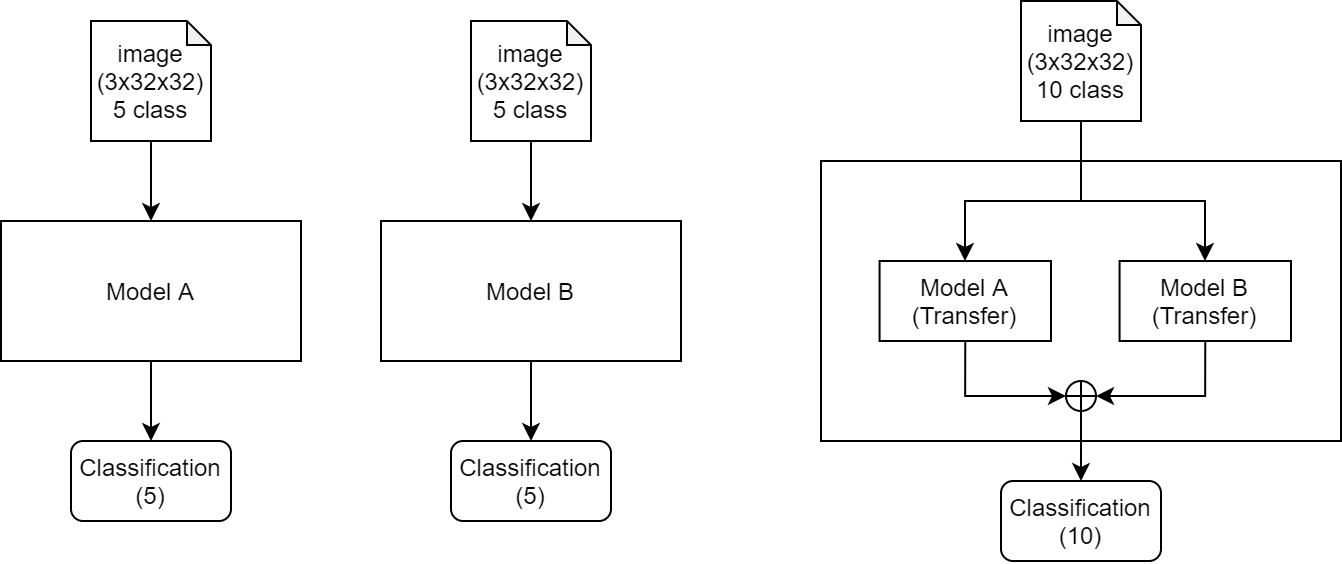
\includegraphics[clip,width=16cm]{model_figure.png}
		\caption{モデルの簡略図 ()内はデータの次元数}
		\label{fig:model}
	\end{center}
\end{figure*}

\subsection{5クラスx2}

cifar10に含まれる10クラスを5クラスずつに分割した。インデックスの前半(airplane, mobile, bird, cat, deer)と後半(dog, frog, horse, ship, truck)で分けることにした。生成した部分データセットを、それぞれモデルA, Bで学習した。5クラス分類ができるモデルA, Bを持つ結合モデルA + Bを作成し、10クラス分類の精度を計測した。このモデルの学習と相互関係を図\ref{fig:model}に示した。

結合モデルA + Bは10クラスのデータセットをA, Bに入力し、得られた出力をクラスインデックス順に結合して、出力とする。結合では特別な処理を行わず、そのままのデータを連結した.

\subsection{7クラスx3}

\begin{table}[tb]
  \begin{center}
    \caption{モデルごとの7クラスの振り分け}
    \begin{tabular}{|c||c|c|c|c|c|c|c|c|c|c|} \hline
      model & 0 & 1 & 2 & 3 & 4 & 5 & 6 & 7 & 8 & 9 \\ \hline\hline
      A     & o & o & o & o & o & o & o & _ & _ & _ \\ \hline
      B     & o & o & o & o & _ & _ & _ & o & o & o \\ \hline
      C     & o & _ & _ & _ & o & o & o & o & o & o \\ \hline
    \end{tabular}
    \label{tab:class7}
  \end{center}
\end{table}

さらに今回は, 細川君に指摘してもらったアイデアでも実験を行った. 7クラス分類器を3つ組み合わせて,10クラスの分類を行った. 表\ref{tab:class7}のように, 2つ以上の分類器で各クラスを推定するように, クラスを振り分けた.

\subsection{結果}

\begin{figure}[tb]
	\begin{center}
		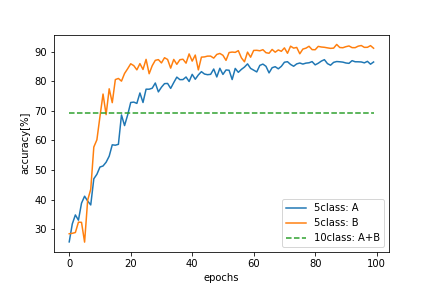
\includegraphics[clip,width=8.5cm]{accuracy5.png}
		\caption{5クラス分類の正答率}
		\label{fig:accuracy5}
	\end{center}
\end{figure}

\begin{figure}[tb]
	\begin{center}
		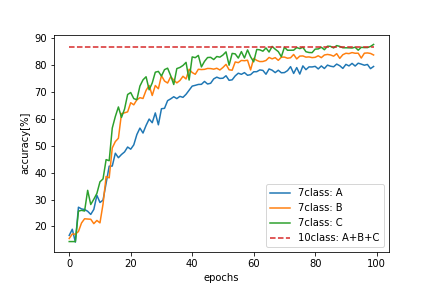
\includegraphics[clip,width=8.5cm]{accuracy7.png}
		\caption{7クラス分類の正答率}
		\label{fig:accuracy7}
	\end{center}
\end{figure}

5クラス分類の精度を図\ref{fig:accuracy5}に, 7クラス分類の精度を図\ref{fig:accuracy7}に示した.

5クラス分類の場合, 80\% ~ 90\%の正答率で前回よりも10\%程向上した. 前回のデータ数2000よりもデータ数を増やしたことで精度がよくなった. 結合した結果も, 70\%(前回+20\%)となった.

7クラス分類では, 正答率が平均80\%程度で, 結合した結果10クラス分類では86.7\%となった.

\section{考察}
% 精度が出ない,とかだけではなく自分なりの考察を示す
データ数とバッチサイズを増やして, 精度の向上と学習の安定化ができた. 特に5クラス分類ではあるが, 正答率 9割を超えることができた. データオーギュメントはしていないので, さらに精度を上げることはできると思われる.

図\ref{fig:accuracy5}, \ref{fig:accuracy7}ともにインデックスが前半のクラスを持つモデルでは, 正答率が低い傾向が見られた. 誤差の影響ではなく, 困難なクラスの分類によって精度が下がっていると考えられる. これはクラスを単純に分割したことによる偏りに原因がある.

分割する組み合わせを自由に替える実装ができたので, 様々な組み合わせパターンで実験して, その差異を見たい.
特にモデル間の正答率の差が目立ったため, これを埋めるような組み合わせを探したい.

\section{今後の予定}
% なんとなくなんかの勉強をするとかではなく具体的に
\begin{itemize}
	\item {クラスの組み合わせの改良}
\end{itemize}


\section{ソースコード}
% 埋め込みでもGitでもいいので参照できるように

結合モデルのPytorchでの実装をコード\ref{model_cnn}に示す.

\begin{lstlisting}[caption=concat,label=model_cnn]
class catCNN(nn.Module):
  def __init__(self, models, device, n_class=10):
    super(catCNN, self).__init__()
    self.models = models
    self.n_class = n_class
    self.device = device

  def forward(self, x):
    batch_size = x.shape[0]
    output = torch.zeros(batch_size, self.n_class).to(self.device)
    count = torch.zeros(self.n_class).to(self.device)
    for idx, model in self.models:
      idx = torch.tensor(idx).to(self.device)
      output.index_add_(1, idx, model(x))
      count[idx] += 1

    output = output / count
    return output
\end{lstlisting}


% 参考文献リスト
\bibliographystyle{unsrt}
\bibliography{ref}
\end{document}
